\documentclass{article}\usepackage[]{graphicx}\usepackage[]{color}
%% maxwidth is the original width if it is less than linewidth
%% otherwise use linewidth (to make sure the graphics do not exceed the margin)
\makeatletter
\def\maxwidth{ %
  \ifdim\Gin@nat@width>\linewidth
    \linewidth
  \else
    \Gin@nat@width
  \fi
}
\makeatother

\definecolor{fgcolor}{rgb}{0.345, 0.345, 0.345}
\newcommand{\hlnum}[1]{\textcolor[rgb]{0.686,0.059,0.569}{#1}}%
\newcommand{\hlstr}[1]{\textcolor[rgb]{0.192,0.494,0.8}{#1}}%
\newcommand{\hlcom}[1]{\textcolor[rgb]{0.678,0.584,0.686}{\textit{#1}}}%
\newcommand{\hlopt}[1]{\textcolor[rgb]{0,0,0}{#1}}%
\newcommand{\hlstd}[1]{\textcolor[rgb]{0.345,0.345,0.345}{#1}}%
\newcommand{\hlkwa}[1]{\textcolor[rgb]{0.161,0.373,0.58}{\textbf{#1}}}%
\newcommand{\hlkwb}[1]{\textcolor[rgb]{0.69,0.353,0.396}{#1}}%
\newcommand{\hlkwc}[1]{\textcolor[rgb]{0.333,0.667,0.333}{#1}}%
\newcommand{\hlkwd}[1]{\textcolor[rgb]{0.737,0.353,0.396}{\textbf{#1}}}%

\usepackage{framed}
\makeatletter
\newenvironment{kframe}{%
 \def\at@end@of@kframe{}%
 \ifinner\ifhmode%
  \def\at@end@of@kframe{\end{minipage}}%
  \begin{minipage}{\columnwidth}%
 \fi\fi%
 \def\FrameCommand##1{\hskip\@totalleftmargin \hskip-\fboxsep
 \colorbox{shadecolor}{##1}\hskip-\fboxsep
     % There is no \\@totalrightmargin, so:
     \hskip-\linewidth \hskip-\@totalleftmargin \hskip\columnwidth}%
 \MakeFramed {\advance\hsize-\width
   \@totalleftmargin\z@ \linewidth\hsize
   \@setminipage}}%
 {\par\unskip\endMakeFramed%
 \at@end@of@kframe}
\makeatother

\definecolor{shadecolor}{rgb}{.97, .97, .97}
\definecolor{messagecolor}{rgb}{0, 0, 0}
\definecolor{warningcolor}{rgb}{1, 0, 1}
\definecolor{errorcolor}{rgb}{1, 0, 0}
\newenvironment{knitrout}{}{} % an empty environment to be redefined in TeX

\usepackage{alltt}

\usepackage[margin = 0.5in]{geometry}
\usepackage{float, enumitem}
\usepackage{graphicx}
\usepackage{amsmath}

\setlength{\topsep}{0pt}
\setlength{\parskip}{0pt}
\setlength{\partopsep}{1pt}

\renewcommand\thesubsection{\thesection (\alph{subsection})}
\IfFileExists{upquote.sty}{\usepackage{upquote}}{}
\begin{document}

\title{ASSIGNMENT 5}
\author{Brandon Lampe \\ STAT 527 \\ Advanced Data Analysis I}
\maketitle

\section{REM with ethanol treatment:}



Load and format data with:

\begin{knitrout}
\definecolor{shadecolor}{rgb}{0.969, 0.969, 0.969}\color{fgcolor}\begin{kframe}
\begin{alltt}
\hlcom{# read table as it appears above, simply copy/paste}
\hlstd{dat1} \hlkwb{<-} \hlkwd{read.table}\hlstd{(}\hlkwc{text}\hlstd{=}\hlstr{"
          0 g/kg 88.6 73.2 91.4 68.0 75.2
          1 g/kg 63.0 53.9 69.2 50.1 71.5
          2 g/kg 44.9 59.5 40.2 56.3 38.7
          4 g/kg 31.0 39.6 45.3 25.2 22.7

"}\hlstd{,} \hlkwc{header}\hlstd{=}\hlnum{FALSE}\hlstd{)}
\hlcom{# extract only columns with data values}
\hlstd{dat2} \hlkwb{<-} \hlstd{dat1[,} \hlnum{3}\hlopt{:}\hlnum{7}\hlstd{]}
\hlcom{# transpose the matrix so each treatment row is now in its own column}
\hlstd{dat3} \hlkwb{<-} \hlkwd{t}\hlstd{(dat2)}
\hlcom{# change matrix to a data.frame}
\hlstd{rem} \hlkwb{<-} \hlkwd{as.data.frame}\hlstd{(dat3)}
\hlcom{# name the columns based on dosage}
\hlkwd{colnames}\hlstd{(rem)} \hlkwb{<-} \hlkwd{c}\hlstd{(}\hlstr{"0"}\hlstd{,} \hlstr{"1"}\hlstd{,} \hlstr{"2"}\hlstd{,} \hlstr{"4"}\hlstd{)}
\hlcom{# Convert to long format}
\hlstd{rem.long} \hlkwb{<-} \hlkwd{melt}\hlstd{(rem,} \hlkwc{variable.name} \hlstd{=} \hlstr{"dose"}\hlstd{,} \hlkwc{value.name} \hlstd{=} \hlstr{"minutes"}\hlstd{)}
\end{alltt}


{\ttfamily\noindent\itshape\color{messagecolor}{\#\# No id variables; using all as measure variables}}\begin{alltt}
\hlcom{# add column to include units of dose}
\hlstd{rem.long}\hlopt{$}\hlstd{Dose} \hlkwb{<-} \hlkwd{rep}\hlstd{(}\hlnum{NA}\hlstd{,} \hlkwd{nrow}\hlstd{(rem.long))}
\hlstd{rem.long[(rem.long}\hlopt{$}\hlstd{dose} \hlopt{==} \hlnum{0}\hlstd{),} \hlstr{"Dose"}\hlstd{]} \hlkwb{<-} \hlstr{"0 g/kg"}
\hlstd{rem.long[(rem.long}\hlopt{$}\hlstd{dose} \hlopt{==} \hlnum{1}\hlstd{),} \hlstr{"Dose"}\hlstd{]} \hlkwb{<-} \hlstr{"1 g/kg"}
\hlstd{rem.long[(rem.long}\hlopt{$}\hlstd{dose} \hlopt{==} \hlnum{2}\hlstd{),} \hlstr{"Dose"}\hlstd{]} \hlkwb{<-} \hlstr{"2 g/kg"}
\hlstd{rem.long[(rem.long}\hlopt{$}\hlstd{dose} \hlopt{==} \hlnum{4}\hlstd{),} \hlstr{"Dose"}\hlstd{]} \hlkwb{<-} \hlstr{"4 g/kg"}
\hlstd{rem.long}\hlopt{$}\hlstd{Dose} \hlkwb{<-} \hlkwd{factor}\hlstd{(rem.long}\hlopt{$}\hlstd{Dose)}
\end{alltt}
\end{kframe}
\end{knitrout}


\subsection{(10 pts) Make an appropriate graphical summary of the data to compare the groups. Compute, the sample means and standard deviations for the 4 treatment groups.}

\begin{knitrout}
\definecolor{shadecolor}{rgb}{0.969, 0.969, 0.969}\color{fgcolor}\begin{kframe}
\begin{alltt}
\hlcom{#create box plot}
\hlstd{dat1.p} \hlkwb{<-} \hlkwd{ggplot}\hlstd{(rem.long,} \hlkwd{aes}\hlstd{(}\hlkwc{x} \hlstd{= Dose,} \hlkwc{y} \hlstd{= minutes))}
\hlcom{# plot global mean}
\hlstd{dat1.p} \hlkwb{<-} \hlstd{dat1.p} \hlopt{+} \hlkwd{geom_hline}\hlstd{(}\hlkwc{yintercept} \hlstd{=} \hlkwd{mean}\hlstd{(rem.long}\hlopt{$}\hlstd{minutes),} \hlkwc{color} \hlstd{=} \hlstr{"black"}\hlstd{,}
                              \hlkwc{linetype} \hlstd{=} \hlstr{"dashed"}\hlstd{,} \hlkwc{size} \hlstd{=} \hlnum{0.3}\hlstd{,}  \hlkwc{alpha} \hlstd{=} \hlnum{0.5}\hlstd{)}
\hlstd{dat1.p} \hlkwb{<-} \hlstd{dat1.p} \hlopt{+} \hlkwd{geom_boxplot}\hlstd{(}\hlkwc{size} \hlstd{=} \hlnum{0.75}\hlstd{,} \hlkwc{alpha} \hlstd{=} \hlnum{0.5}\hlstd{)} \hlcom{# boxplot}
\hlstd{dat1.p} \hlkwb{<-} \hlstd{dat1.p} \hlopt{+} \hlkwd{geom_point}\hlstd{(}\hlkwc{position} \hlstd{=} \hlkwd{position_jitter}\hlstd{(}\hlkwc{w} \hlstd{=} \hlnum{0.05}\hlstd{,} \hlkwc{h} \hlstd{=} \hlnum{0}\hlstd{),}
                              \hlkwc{alpha} \hlstd{=} \hlnum{0.5}\hlstd{,} \hlkwc{size} \hlstd{=} \hlnum{2}\hlstd{)}
\hlstd{dat1.p} \hlkwb{<-} \hlstd{dat1.p} \hlopt{+} \hlkwd{stat_summary}\hlstd{(}\hlkwc{fun.y} \hlstd{= mean,} \hlkwc{geom} \hlstd{=} \hlstr{"point"}\hlstd{,} \hlkwc{shape} \hlstd{=} \hlnum{18}\hlstd{,}
                                \hlkwc{size} \hlstd{=} \hlnum{6}\hlstd{,} \hlkwd{aes}\hlstd{(}\hlkwc{color} \hlstd{= Dose),} \hlkwc{alpha} \hlstd{=} \hlnum{0.8}\hlstd{)}
\hlstd{dat1.p} \hlkwb{<-} \hlstd{dat1.p} \hlopt{+} \hlkwd{stat_summary}\hlstd{(}\hlkwc{fun.data} \hlstd{=} \hlstr{"mean_cl_normal"}\hlstd{,} \hlkwc{geom} \hlstd{=} \hlstr{"errorbar"}\hlstd{,}
                                \hlkwc{width} \hlstd{=} \hlnum{.1}\hlstd{,} \hlkwd{aes}\hlstd{(}\hlkwc{color} \hlstd{= Dose),} \hlkwc{alpha} \hlstd{=} \hlnum{0.8}\hlstd{)}

\hlstd{dat1.p} \hlkwb{<-} \hlstd{dat1.p} \hlopt{+} \hlkwd{labs}\hlstd{(}\hlkwc{y} \hlstd{=}\hlstr{"REM Sleep Duration (minute)"}\hlstd{,}\hlkwc{x} \hlstd{=} \hlstr{"Dose"}\hlstd{)}

\hlstd{dat1.p} \hlkwb{<-} \hlstd{dat1.p} \hlopt{+} \hlkwd{guides}\hlstd{(}\hlkwc{color} \hlstd{=} \hlnum{FALSE}\hlstd{)}
\hlcom{# create histograms}
\hlstd{dat1.hist} \hlkwb{<-} \hlkwd{ggplot}\hlstd{(rem.long,} \hlkwd{aes}\hlstd{(}\hlkwc{x} \hlstd{= minutes))} \hlopt{+} \hlkwd{geom_histogram}\hlstd{(}\hlkwc{binwidth} \hlstd{=} \hlnum{10}\hlstd{)}
\hlstd{dat1.hist} \hlkwb{<-} \hlstd{dat1.hist} \hlopt{+} \hlkwd{facet_grid}\hlstd{(Dose} \hlopt{~} \hlstd{.)}
\hlstd{dat1.hist} \hlkwb{<-} \hlstd{dat1.hist}\hlopt{+} \hlkwd{labs}\hlstd{(}\hlkwc{y} \hlstd{=} \hlstr{"Count"}\hlstd{,} \hlkwc{x} \hlstd{=} \hlstr{"REM Sleep Duration (minutes)"}\hlstd{)}
\hlcom{# plot boxplot and historgram}
\hlkwd{grid.arrange}\hlstd{(dat1.p, dat1.hist,} \hlkwc{ncol} \hlstd{=} \hlnum{2}\hlstd{)}
\end{alltt}
\end{kframe}\begin{figure}[]


{\centering 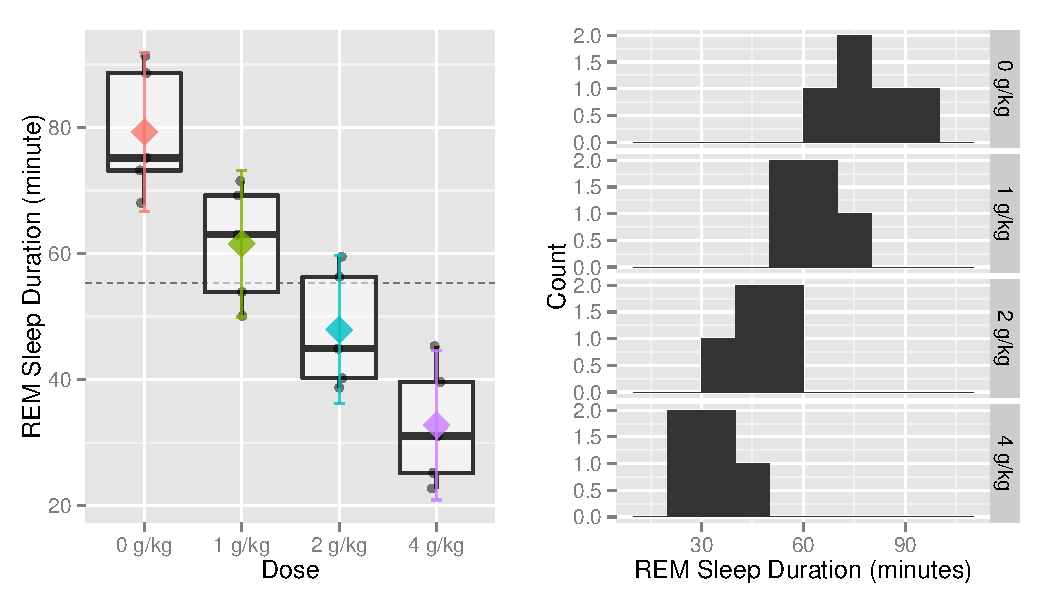
\includegraphics[width=\maxwidth]{figure/a_BoxPlot-1} 

}

\caption[REM Sleep Duration Summary for Each Treatment of Ethanol (g of Ethanol per kg of Body Mass)]{REM Sleep Duration Summary for Each Treatment of Ethanol (g of Ethanol per kg of Body Mass).\label{fig:a_BoxPlot}}
\end{figure}


\end{knitrout}

\begin{knitrout}
\definecolor{shadecolor}{rgb}{0.969, 0.969, 0.969}\color{fgcolor}\begin{kframe}
\begin{alltt}
\hlcom{# global mean}
\hlstd{Yglob} \hlkwb{<-} \hlkwd{mean}\hlstd{(rem.long}\hlopt{$}\hlstd{minutes)} \hlcom{# because each sample is the same size}
\hlstd{Yglob}
\end{alltt}
\begin{verbatim}
## [1] 55.375
\end{verbatim}
\begin{alltt}
\hlstd{stats} \hlkwb{<-} \hlkwd{data.frame}\hlstd{(}\hlkwd{ddply}\hlstd{(rem.long,} \hlkwd{.}\hlstd{(dose), summarize,} \hlkwc{mean} \hlstd{=} \hlkwd{round}\hlstd{(}\hlkwd{mean}\hlstd{(minutes),} \hlnum{1}\hlstd{),}
               \hlkwc{sd} \hlstd{=} \hlkwd{round}\hlstd{(}\hlkwd{sd}\hlstd{(minutes),} \hlnum{1}\hlstd{),} \hlkwc{spread} \hlstd{=} \hlkwd{round}\hlstd{(}\hlkwd{max}\hlstd{(minutes)} \hlopt{-} \hlkwd{min}\hlstd{(minutes)),}
               \hlkwc{iqr} \hlstd{=} \hlkwd{IQR}\hlstd{(minutes),} \hlkwc{sdOut} \hlstd{=} \hlkwd{round}\hlstd{((Yglob} \hlopt{-} \hlkwd{mean}\hlstd{(minutes))}\hlopt{/}\hlkwd{sd}\hlstd{(minutes),}\hlnum{1}\hlstd{)))}
\end{alltt}


{\ttfamily\noindent\bfseries\color{errorcolor}{\#\# Error in eval(expr, envir, enclos): argument "{}by"{} is missing, with no default}}\begin{alltt}
\hlstd{stats} \hlcom{#error message is associated with KnitR bug... evaluation works fine in R}
\end{alltt}


{\ttfamily\noindent\bfseries\color{errorcolor}{\#\# Error in eval(expr, envir, enclos): object 'stats' not found}}\end{kframe}
\end{knitrout}
\vspace{.25in}
\begin{center}
\begin{tabular}{c c c}
  Treatment Group & Mean & Standard Deviation \\ \hline
  0 & 79.3 & 10.2 \\
  1 & 61.5 & 9.3 \\
  2 & 47.9 & 9.5 \\
  4 & 32.8 & 9.6 \\ \hline
\end{tabular}
\end{center}
\vspace{.1in}

Each of the five samples only contain 5 data points, which makes assessing normality difficult to disprove.  The global mean is 55.4, and the spread and IQR for each of samples are nearly identical as they vary by less than 5\%.

\subsection{(10 pts) Looking at the graphical and descriptive summaries from part (a), do there appear to be differences in the typical REM levels for the 4 groups? Describe the differences you see that appear to be most pronounced.}

Yes, there appear to be differences in the typical REM levels fro the 4 groups.  Differences exist in the value of each samples mean and the relative distance of the sample mean to the global mean.  Adjacent groups appear have similar means; however, groups that are not adjacent do not appear to have similar means.  Only groups 1 and 2 have IQRs that include the global mean, while groups 0 and 4 do not even have outliers that cross the global mean.

Below is a summary of confidence levels and sample means relative to the global mean:

\begin{itemize}
  \item Treatment Group 0:  The 95\% confidence level of the sample mean does not include the global mean.  The global mean is less than the sample mean by 2.3 standard deviations of the sample mean.
  \item Treatment Group 1:  The 95\% confidence level of the sample mean does include the global mean and is within 0.7 standard deviations of the sample mean.
  \item Treatment Group 2:  The 95\% confidence level of the sample mean does include the global mean and is within 0.8 standard deviations of the sample mean.
  \item Treatment Group 4:  The 95\% confidence level of the sample mean does not include the global mean.  The global mean is greater than the sample mean by 2.4 standard deviations of the sample mean.
\end{itemize}

\subsection{(10 pts) Do a one-way Analysis of Variance to compare the mean REM levels for the 4 groups. Are the groups significantly different at the 5\% level?}

\begin{knitrout}
\definecolor{shadecolor}{rgb}{0.969, 0.969, 0.969}\color{fgcolor}\begin{kframe}
\begin{alltt}
\hlcom{# perform ANalaysi Of VAriance}
\hlstd{fit.REM} \hlkwb{<-} \hlkwd{aov}\hlstd{(minutes} \hlopt{~} \hlstd{dose,} \hlkwc{data} \hlstd{= rem.long)}
\hlkwd{summary}\hlstd{(fit.REM)}
\end{alltt}
\begin{verbatim}
##             Df Sum Sq Mean Sq F value   Pr(>F)    
## dose         3   5882    1961   21.09 8.32e-06 ***
## Residuals   16   1487      93                     
## ---
## Signif. codes:  0 '***' 0.001 '**' 0.01 '*' 0.05 '.' 0.1 ' ' 1
\end{verbatim}
\begin{alltt}
\hlstd{fit.REM}
\end{alltt}
\begin{verbatim}
## Call:
##    aov(formula = minutes ~ dose, data = rem.long)
## 
## Terms:
##                     dose Residuals
## Sum of Squares  5882.358  1487.400
## Deg. of Freedom        3        16
## 
## Residual standard error: 9.641706
## Estimated effects may be unbalanced
\end{verbatim}
\end{kframe}
\end{knitrout}
\begin{itemize}
\item The population parameter for each sample is the mean REM sleep duration, $\mu_n = $ average sleep duration for sample $n$.

\item The F-statistic is used to test if it is plausible that the mean REM sleep durations of the four samples are all equal; that is $H_0: \mu_1 = \mu_2 = \mu_3 = \mu_4$.  Where the alternative is that any two or more of the mean REM sleep durations are not equal; that is $H_A:$ not $H_0$.

\item The p-value of the F-test is 8.3e-6; therefore, I reject the Null hypothesis in favor of the Alternative hypothesis.  The mean REM sleep durations of the four populations are not all equal at the 5\% level or even the 1\% level.

\end{itemize}

\subsection{(10 pts) Compare all possible pairs of groups using Fisher’s LSD method, and summarize the results of the multiple comparison. Repeat for Tukey’s HSD method, and using Bonferroni comparisons. Do the three methods find different groupings? If so, what accounts for that?}

\begin{knitrout}
\definecolor{shadecolor}{rgb}{0.969, 0.969, 0.969}\color{fgcolor}\begin{kframe}
\begin{alltt}
\hlstd{n.sample} \hlkwb{<-} \hlnum{4} \hlcom{# number of population samples for which a mean was taken}

\hlcom{# family error rate:  alpha < FER < c*alpha}
\hlstd{alpha} \hlkwb{<-} \hlnum{0.05}
\hlstd{c} \hlkwb{<-} \hlstd{n.sample}\hlopt{*}\hlstd{(n.sample}\hlopt{-}\hlnum{1}\hlstd{)}\hlopt{/}\hlnum{2} \hlcom{#pairs of means to compare}
\hlstd{c}\hlopt{*}\hlstd{alpha}
\end{alltt}
\begin{verbatim}
## [1] 0.3
\end{verbatim}
\begin{alltt}
\hlcom{# Fisher's LSD method}
\hlkwd{pairwise.t.test}\hlstd{(rem.long}\hlopt{$}\hlstd{minutes, rem.long}\hlopt{$}\hlstd{dose,} \hlkwc{pool.sd} \hlstd{=} \hlnum{TRUE}\hlstd{,} \hlkwc{p.adjust.method} \hlstd{=} \hlstr{"none"}\hlstd{)}
\end{alltt}
\begin{verbatim}
## 
## 	Pairwise comparisons using t tests with pooled SD 
## 
## data:  rem.long$minutes and rem.long$dose 
## 
##   0       1       2      
## 1 0.01024 -       -      
## 2 9.8e-05 0.04014 -      
## 4 1.0e-06 0.00023 0.02435
## 
## P value adjustment method: none
\end{verbatim}
\end{kframe}
\end{knitrout}
\textbf{Fisher's LSD Method:}  At the 5\% level, sufficient eveidence exists to conclude that all populations means are unique.  Results from this analysis are shown below in groups, notice that no groups are paired.

\begin{verbatim}
4 g/kg     2 g/kg     1 g/kg     0 g/kg
------     ------     ------     ------
\end{verbatim}\

Family Error Rate:  $\alpha < FER < c \alpha \rightarrow 0.05 < FER < 0.30$\\

\begin{knitrout}
\definecolor{shadecolor}{rgb}{0.969, 0.969, 0.969}\color{fgcolor}\begin{kframe}
\begin{alltt}
\hlcom{# Tukey's HSD method}
\hlkwd{TukeyHSD}\hlstd{(fit.REM)}
\end{alltt}
\begin{verbatim}
##   Tukey multiple comparisons of means
##     95% family-wise confidence level
## 
## Fit: aov(formula = minutes ~ dose, data = rem.long)
## 
## $dose
##       diff       lwr         upr     p adj
## 1-0 -17.74 -35.18636  -0.2936428 0.0455781
## 2-0 -31.36 -48.80636 -13.9136428 0.0005142
## 4-0 -46.52 -63.96636 -29.0736428 0.0000056
## 2-1 -13.62 -31.06636   3.8263572 0.1563545
## 4-1 -28.78 -46.22636 -11.3336428 0.0011925
## 4-2 -15.16 -32.60636   2.2863572 0.1005398
\end{verbatim}
\end{kframe}
\end{knitrout}
\textbf{Tukey's HSD Method:}  At the 5\% level, insufficient evidence exists to conclude that the population mean REM sleep duration for 1 g/Kg dosage, 2 g/Kg dosage, and 4 g/Kg dosage are unique.  Sufficient evidence exists to conclude the mean REM sleep duration for 0 g/Kg dosage is different from the other populations means at the 5\% level.  Additionally, sufficient evidence exists to conclude the population mean REM sleep durations of 4 g/Kg and 1 g/Kg are different at the 5\% level. Results from this analysis are shown below in groups.

\begin{verbatim}
4 g/kg     2 g/kg     1 g/kg     0 g/kg
           ------------------
-----------------
\end{verbatim}

Family Error Rate:  varies\\


\begin{knitrout}
\definecolor{shadecolor}{rgb}{0.969, 0.969, 0.969}\color{fgcolor}\begin{kframe}
\begin{alltt}
\hlcom{# family error rate:  alpha/c < FER < alpha}
\hlstd{alpha}\hlopt{/}\hlstd{c} \hlcom{# lower bound}
\end{alltt}
\begin{verbatim}
## [1] 0.008333333
\end{verbatim}
\begin{alltt}
\hlstd{alpha} \hlcom{# upper bound}
\end{alltt}
\begin{verbatim}
## [1] 0.05
\end{verbatim}
\begin{alltt}
\hlcom{# Bonferroni comparison method}
\hlkwd{pairwise.t.test}\hlstd{(rem.long}\hlopt{$}\hlstd{minutes, rem.long}\hlopt{$}\hlstd{dose,} \hlkwc{pool.sd} \hlstd{=} \hlnum{TRUE}\hlstd{,} \hlkwc{p.adjust.method} \hlstd{=} \hlstr{"bonf"}\hlstd{)}
\end{alltt}
\begin{verbatim}
## 
## 	Pairwise comparisons using t tests with pooled SD 
## 
## data:  rem.long$minutes and rem.long$dose 
## 
##   0       1       2      
## 1 0.06146 -       -      
## 2 0.00059 0.24085 -      
## 4 6.1e-06 0.00139 0.14608
## 
## P value adjustment method: bonferroni
\end{verbatim}
\end{kframe}
\end{knitrout}
\textbf{Bonferroni Comparison Method:}  At the 5\% level, insufficient evidence exists to conclue that the population mean REM sleep durations of 1 g/Kg dosage and 2 g/Kg dosage, 2 g/Kg dosage and 4 g/Kg dosage, and 1 g/Kg dosage and 0 g/Kg dosage are different.  Sufficent evidence exists to conclude the population mean REM sleep durations of 4 g/Kg differ from 1 and 0 g/Kg and that 2 g/Kg differ from 0 g/Kg. Results from this analysis are shown below in groups.

\begin{verbatim}
4 g/kg     2 g/kg     1 g/kg     0 g/kg
                      -----------------
          ------------------
-----------------
\end{verbatim}\

Family Error Rate:  $\alpha/c < FER < \alpha \rightarrow 0.0083 < FER < 0.05$\\

\textbf{Do the methods find different groupings?}  Yes, Fisher's method did not result in any groupings, Tukey's method resulted in two groupings, and Bonferroni's methods resulted in three groupings. Of the methods utilized, Fisher's Method is the most likely to result in a Type I error (reject a true null hypothesis) as it is the most liberal of the three.  Bonferroni's method is the most conservative of the three methods and is most likely to reult in a Type II error (fail to reject a false null hypothesis).  Regarding error, Tukey's method falls in between the other two methods as its erorr is equal to a t-test but it accounts for increased probability of making a Type I error when making multiple comparisons.  Tukey's method feels right.

\subsection{(10 pts) Are the results of the F -test in part (c), and the multiple comparisons in part (d) consistent with what you described in part (b)? Briefly discuss.}
Results from the F-test in part (c) are consistent with what I described in part (b).  That is, at the 5\% level (approximately two standard deviations) the groups do not all have the same mean.  Results in part (d) are not consistent with what I described in part (b).  I was unable to distinguish paired groups (those with similar means at the 5\% level) based on a graphical summary.  Adjacent groups appear to have similar differences between ranges, IQRs, means, and medians.  However, Tukey's method identified two sets of paired groups where I was unable to distinguish this in part (b).

\subsection{(10pts) Looking at the numerical and graphical summaries does it appear that the distributions of REM levels are reasonably normal, and have constant variance across groups? Discuss.}
Based on the histogram and box plots in part (b), the distributions of the REM levels appear normal have have nearly constant variance across each group.  The spread and standard deviation of each group varies by less than 5\% across all the sample data.

\subsection{(10 pts) Comment on the Levene’s and Bartlett’s formal tests of equal variances in light of what you see when you look at the data.}

\begin{knitrout}
\definecolor{shadecolor}{rgb}{0.969, 0.969, 0.969}\color{fgcolor}\begin{kframe}
\begin{alltt}
\hlcom{#Bartlett's test of equal variances}
\hlkwd{bartlett.test}\hlstd{(minutes} \hlopt{~} \hlstd{dose,} \hlkwc{data} \hlstd{= rem.long)}
\end{alltt}
\begin{verbatim}
## 
## 	Bartlett test of homogeneity of variances
## 
## data:  minutes by dose
## Bartlett's K-squared = 0.0323, df = 3, p-value = 0.9985
\end{verbatim}
\begin{alltt}
\hlcom{#Levene's test of equal variances}
\hlkwd{leveneTest}\hlstd{(minutes} \hlopt{~} \hlstd{dose,} \hlkwc{data} \hlstd{= rem.long)}
\end{alltt}
\begin{verbatim}
## Levene's Test for Homogeneity of Variance (center = median)
##       Df F value Pr(>F)
## group  3  0.0058 0.9994
##       16
\end{verbatim}
\end{kframe}
\end{knitrout}
The Bartlett and Levene tests both have the null hypothesis that sample distributions all have equal variance and alternate hypothesis that at least one sample distribution variance is not equal to the variance of another sample.  Results from both the Bartlett and Levene tests fail to reject the Null hypothesis of the tests.  P-values of both the Bartlett and Levene tests are well above 0.05, 0.9985 and 0.994, respectively.  Therefore, at the 5\% level and 1\% level insufficient evidence exists to conclude the four samples are from poulations with an unequal variance.  These results agree with the inference made based on the calculated standard deviations, i.e., the variances are equal.\\

The Bartlett's test is sensitive to departures from normality where Levene's test is less sensitive to departures from normality.  The histogram of data does not appear normal, but the symmetry shown in the box plots does indicate the data are normal.  The normality assumption should be verified for these tests.

\subsection{(10 pts) Obtain the residuals (or centered values) and generate a normal probability plot based on them. This is an overall check on normality. Is the normality assumption reasonable here? Perform a formal test of normality on the residuals, report the p-value and comment. If the test says we did not sample from normally distributed populations, why does it appear to be saying that? Do you think there is a real difficulty here with applying the normal theory methods?}

\begin{knitrout}
\definecolor{shadecolor}{rgb}{0.969, 0.969, 0.969}\color{fgcolor}\begin{kframe}
\begin{alltt}
\hlcom{# create histograms}
\hlstd{resid} \hlkwb{<-} \hlkwd{data.frame}\hlstd{(fit.REM}\hlopt{$}\hlstd{residuals)}
\hlkwd{colnames}\hlstd{(resid)} \hlkwb{<-} \hlstr{"r"}

\hlcom{# create histograms}
\hlstd{resid.hist} \hlkwb{<-} \hlkwd{ggplot}\hlstd{(resid,} \hlkwd{aes}\hlstd{(}\hlkwc{x} \hlstd{= r))}
\hlstd{resid.hist} \hlkwb{<-} \hlstd{resid.hist} \hlopt{+} \hlkwd{scale_x_continuous}\hlstd{(}\hlkwc{limits} \hlstd{=} \hlkwd{c}\hlstd{(}\hlopt{-}\hlnum{15}\hlstd{,}\hlnum{15}\hlstd{))}
\hlstd{resid.hist} \hlkwb{<-} \hlstd{resid.hist} \hlopt{+} \hlkwd{geom_histogram}\hlstd{(}\hlkwc{binwidth} \hlstd{=} \hlnum{4}\hlstd{,} \hlkwc{color} \hlstd{=} \hlstr{"black"}\hlstd{,} \hlkwc{fill} \hlstd{=} \hlstr{"white"}\hlstd{,}
                                          \hlkwd{aes}\hlstd{(}\hlkwc{y} \hlstd{= ..density..))}
\hlstd{resid.hist} \hlkwb{<-} \hlstd{resid.hist} \hlopt{+} \hlkwd{geom_density}\hlstd{(}\hlkwc{alpha} \hlstd{=} \hlnum{0.1}\hlstd{,} \hlkwc{fill} \hlstd{=} \hlstr{"#FF6666"}\hlstd{)}
\hlstd{resid.hist} \hlkwb{<-} \hlstd{resid.hist} \hlopt{+} \hlkwd{labs}\hlstd{(}\hlkwc{y} \hlstd{=} \hlstr{"Count"}\hlstd{,} \hlkwc{x} \hlstd{=} \hlstr{"Residuals of REM Sleep Duration (minutes)"}\hlstd{)}

\hlcom{# boxplot of Unseeded Precip}
\hlstd{resid.box} \hlkwb{<-} \hlkwd{ggplot}\hlstd{(resid,} \hlkwd{aes}\hlstd{(}\hlkwc{x} \hlstd{=} \hlstr{"ANOVA Residuals"}\hlstd{,} \hlkwc{y} \hlstd{= r))} \hlcom{# boxplot}
\hlstd{resid.box} \hlkwb{<-} \hlstd{resid.box} \hlopt{+} \hlkwd{geom_boxplot}\hlstd{()}
\hlstd{resid.box} \hlkwb{<-} \hlstd{resid.box} \hlopt{+} \hlkwd{coord_flip}\hlstd{()}
\hlstd{resid.box} \hlkwb{<-} \hlstd{resid.box} \hlopt{+} \hlkwd{stat_summary}\hlstd{(}\hlkwc{fun.y} \hlstd{= mean,} \hlkwc{geom} \hlstd{=} \hlstr{"point"}\hlstd{,} \hlkwc{shape} \hlstd{=} \hlnum{3}\hlstd{,} \hlkwc{size} \hlstd{=} \hlnum{4}\hlstd{)}
\hlstd{resid.box} \hlkwb{<-} \hlstd{resid.box} \hlopt{+} \hlkwd{geom_point}\hlstd{(}\hlkwc{position} \hlstd{=} \hlkwd{position_jitter}\hlstd{(}\hlkwc{w} \hlstd{=} \hlnum{0.05}\hlstd{,} \hlkwc{h} \hlstd{=} \hlnum{0}\hlstd{),}
                              \hlkwc{alpha} \hlstd{=} \hlnum{0.5}\hlstd{,} \hlkwc{size} \hlstd{=} \hlnum{2}\hlstd{)}
\hlstd{resid.box} \hlkwb{<-} \hlstd{resid.box} \hlopt{+} \hlkwd{labs}\hlstd{(}\hlkwc{y} \hlstd{=} \hlstr{"ANOVA Residuals"}\hlstd{,} \hlkwc{x} \hlstd{=} \hlstr{""}\hlstd{)}

\hlkwd{grid.arrange}\hlstd{(resid.hist, resid.box,} \hlkwc{nrow} \hlstd{=} \hlnum{2}\hlstd{)}
\end{alltt}
\end{kframe}

{\centering 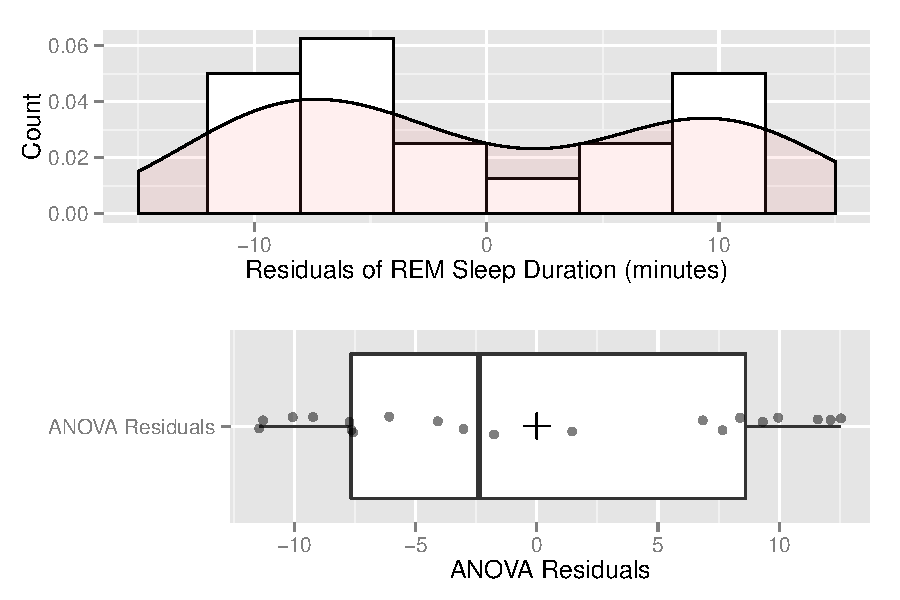
\includegraphics[width=\maxwidth]{figure/h_plot-1} 

}



\end{knitrout}

\begin{knitrout}
\definecolor{shadecolor}{rgb}{0.969, 0.969, 0.969}\color{fgcolor}\begin{kframe}
\begin{alltt}
\hlcom{# QQ plot of residuals (normal probability plot of residuals)}
\hlkwd{qqPlot}\hlstd{(fit.REM}\hlopt{$}\hlstd{residuals,} \hlkwc{las} \hlstd{=} \hlnum{1}\hlstd{,} \hlkwc{id.n} \hlstd{=} \hlnum{8}\hlstd{,} \hlkwc{id.cex} \hlstd{=} \hlnum{1}\hlstd{,} \hlkwc{lwd} \hlstd{=} \hlnum{1}\hlstd{,} \hlkwc{main} \hlstd{=} \hlstr{"QQ Plot of Residuals"}\hlstd{)}
\end{alltt}
\end{kframe}

{\centering 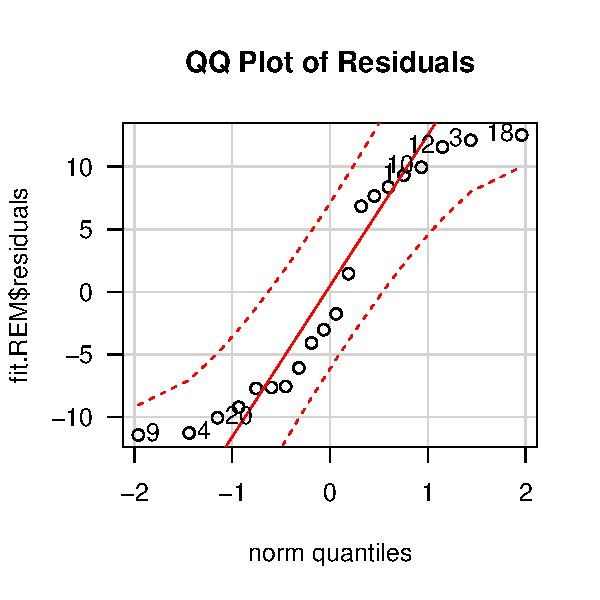
\includegraphics[width=\maxwidth]{figure/h_qq-1} 

}


\begin{kframe}\begin{verbatim}
## 18  3 12  9  4 20 10  1 
## 20 19 18  1  2  3 17 16
\end{verbatim}
\end{kframe}
\end{knitrout}

\begin{knitrout}
\definecolor{shadecolor}{rgb}{0.969, 0.969, 0.969}\color{fgcolor}\begin{kframe}
\begin{alltt}
\hlcom{# shapiro-wilk test for normality}
\hlkwd{shapiro.test}\hlstd{(fit.REM}\hlopt{$}\hlstd{residuals)}
\end{alltt}
\begin{verbatim}
## 
## 	Shapiro-Wilk normality test
## 
## data:  fit.REM$residuals
## W = 0.8781, p-value = 0.01633
\end{verbatim}
\begin{alltt}
\hlcom{# anderson - darling test for normality}
\hlkwd{library}\hlstd{(nortest)}
\hlkwd{ad.test}\hlstd{(fit.REM}\hlopt{$}\hlstd{residuals)}
\end{alltt}
\begin{verbatim}
## 
## 	Anderson-Darling normality test
## 
## data:  fit.REM$residuals
## A = 0.9091, p-value = 0.01651
\end{verbatim}
\end{kframe}
\end{knitrout}
\vspace{0.25in}
\textbf{Historgram and Boxplot of Residuals (data centered about the global mean):}
These plots show the residuals are potentially bimodal, although very few observations were made, which may result in a misleading distribution of the residuals.  The residual distribution is symmetric about the mean.  The mean is near the median and distribution has equal length tails, which are indications of a normal distribution of residuals.\\

\textbf{Normal Probability Plot}
The QQ plot shows that all values fall within the normal distibution at the 5\% level; therefore, there is no evidence from this plot that the residuals deviate from normality at this leve.\\

\textbf{Formal Normality Tests:}
The Shapiro-Wilks and Anderson-Darling tests both have the null hypothesis that the samples are normally distributed and an alternate hypothesis of the samples not being normally distributed.  Both of these tests reject the Null (residuals are not normally distributed) at the 5\% level but fail to reject the Null (residuals are normally distributed) at 1\% level.  The tests appears to be rejecting the Null at the 5\% level because of the small sample sizes, and I think the normal theory methods are suitable for this analysis.



\end{document}
